\section{Introdução}

Ordenar objetos, de uma maneira geral, é bastante útil pois ajuda a
organizar, buscar de forma rápida, verificar existência, entre outros
aspectos. Em computação isso não é diferente. A ordenação é utilizada em
várias áreas, por exemplo Bancos de Dados. Com isso precisamos sempre de
algoritmos de ordenação que façam o trabalho em menos tempo, consumindo
menos recursos.

\section{Métodos de Ordenação}

Para ordenar dados computacionais precisamos de métodos, que consistem
em procedimentos que dado um conjunto geram uma saída com o próximo
elemento sempre menor ou igual ao anterior, ou vice versa.

Veremos a implementação e estatísticas dos seguintes métodos de
ordenação:

\begin{itemize}
\item
  Bubble Sort
\item
  Selection Sort
\item
  Insertion Sort
\item
  Quick Sort
\item
  Counting Sort
\item
  Radix Sort
\end{itemize}
\subsection{Bubble Sort}

Método de ordenação bastante simples de implementar e entender. A ideia
é percorrer um vetor de dados, normalmente números, e verificar de dois
em dois qual o maior. Em caso positivo trocar um com o outro.

\subsubsection{Complexidade}

Para cada elemento é preciso percorrer o vetor, mesmo que o mesmo já
esteja ordenado. Por isso dizemos que o algoritmo é $O(n^2)$.

\subsubsection{Pseudo-código}

Esse método é caracterizado pelo uso de variável auxiliar para fazer o
\emph{swap} ou troca.

\begin{verbatim}
void bubble_sort(V[], n)
begin
    k = n - 1
    for i = 1 to n do
        for j = 0 to k do
            if V[j] > V[j + 1] do
                aux = V[j]
                V[j] = V[j + 1]
                V[j + 1] = aux
            endif
        endfor
    endfor
end
\end{verbatim}
\subsection{Selection Sort}

O algoritmo inicia buscando o valor mínimo e o coloca na primeira
posição. Depois busca o segundo menor valor e o coloca na segunda
posição. Assim por diante.

\subsubsection{Complexidade}

Selecionar o menor elemento requer verificar todos os $n$ elementos
(sendo $n - 1$ comparações) e então colocá-lo na posição correta.
Encontrar o próximo requer uma busca em $n - 1$ elementos. Daí temos:

\begin{equation}
(n - 1) + (n - 2) + \cdots + 2 + 1 = \frac{n (n - 1)}{2} \in \Theta(n^2)
\end{equation}

\subsubsection{Pseudo-código}

Também possui o \emph{swap}, entretanto pode ser que o elemento já
esteja na posição correta, e deverá ser ignorado.

\begin{verbatim}
void selection_sort(V[], n)
begin
    for i = 0 to n - 1 do
        min = i
        for j = i + 1 to n do
            if V[j] < V[min] do
                min = j
            endif
        endfor
        if min != i do
            aux = V[i]
            V[i] = V[min]
            V[min] = aux
        endif
    endfor
end
\end{verbatim}
\subsection{Insertion Sort}

A ideia é, se os primeiros elementos já estão ordenados, um elemento não
ordenado pode ser inserido no conjunto ordenado no lugar adequado.

\subsubsection{Complexidade}

Para inserir o último elemento precisamos de pelo menos $n - 1$
comparações e $n - 1$ movimentos. Para inserir o penúltimo elemento
precisamos de $n - 2$ comparações e $n - 2$ movimentos. E assim por
diante. Daí podemos concluir que teremos:

\begin{equation}
2 \cdot (1 + 2 + 3 + \dots + (n - 1)) = \frac{2 \cdot (n - 1) \cdot n}{2} = (n - 1) \cdot n \in \Theta(n^2)
\end{equation}

\subsubsection{Pseudo-código}

\begin{verbatim}
void insertion_sort(V[], n)
begin
    for i = 1 to n do
        j = i
        while j != 0
                && V[j] < V[j - 1] do
            aux = V[j]
            V[j - 1] = V[j]
            V[j] = aux
            j = j - 1
        endwhile
    endfor
end
\end{verbatim}
\subsection{Counting Sort}

Diferente de todos os algoritmos vistos até aqui, esse algoritmo não usa
comparações. Para a ordenação é preciso contar quantos elementos existem
e colocá-los num array temporário onde o índice do mesmo é o valor e
cada índice representa o número de vezes que aquele valor aparece.

\subsubsection{Complexidade}

\subsubsection{Pseudo-código}

\begin{verbatim}
void counting_sort(V[], n, maxValue)
begin
    count[] = [maxValue + 1]
    for i = 0 to n do
        count[i] = count[i] + 1
    endfor

    z = 0
    for i = 0 to maxValue do
        while count[i] > 0 do
            V[z] = i
            z = z + 1
            count[i] = count[i] - 1
        endwhile
    endfor
end
\end{verbatim}
\subsection{Radix Sort}

\subsubsection{Complexidade}

\subsubsection{Pseudo-código}

\newpage

\subsection{Algoritmo Proposto - Busca do maior e menor}

Inicialmente definimos onde o maior e o menor elementos serão colocados,
usando as variáveis \texttt{ordEsq} e \texttt{ordDir}.

\begin{figure}[h]
   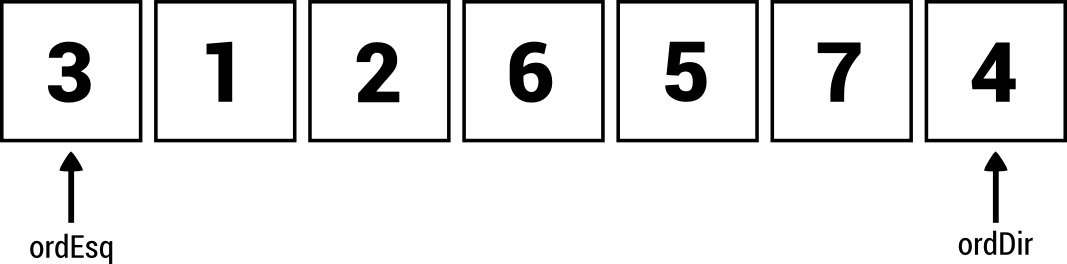
\includegraphics[scale=0.6]{img/maior.menor.algoritmo/passo1.png}
\end{figure}

Logo em seguida fazemos uma busca procurando o maior e o menor
elementos.

\begin{figure}[h]
   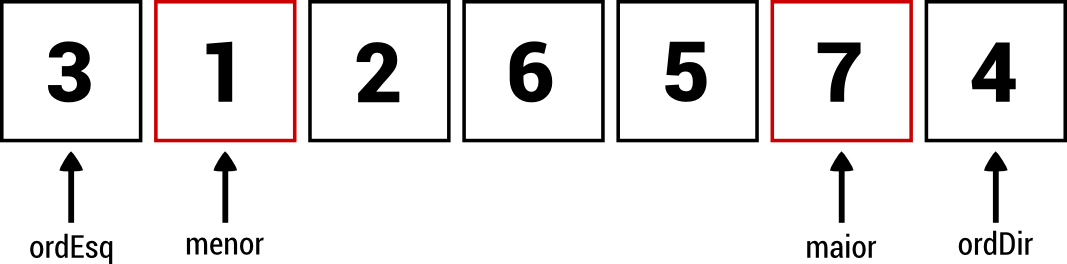
\includegraphics[scale=0.6]{img/maior.menor.algoritmo/passo2.png}
\end{figure}

Ao encontrar devemos trocar o \texttt{menor} com \texttt{ordEsq} e
\texttt{maior} com \texttt{ordDir}. Logo em seguida incrementar o valor
de \texttt{ordEsq} e decrementar o valor de \texttt{ordDir}.

\begin{figure}[h]
   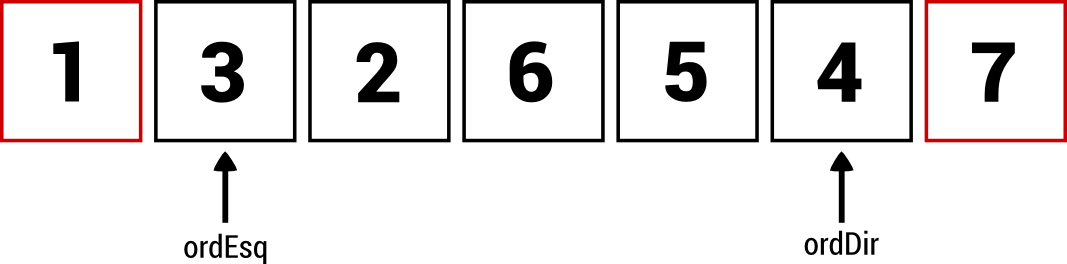
\includegraphics[scale=0.6]{img/maior.menor.algoritmo/passo3.png}
\end{figure}

\newpage

\begin{figure}[h]
   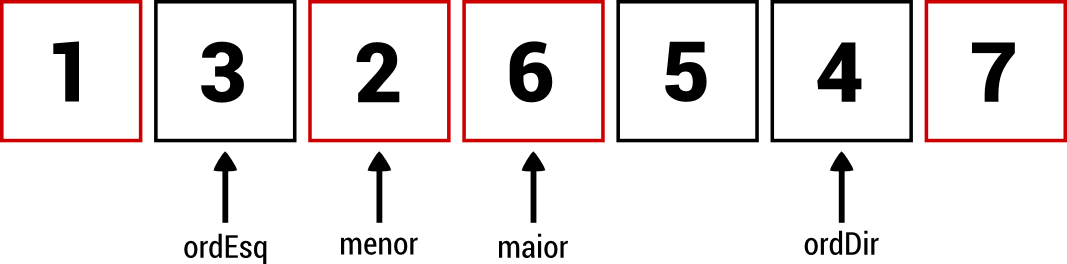
\includegraphics[scale=0.6]{img/maior.menor.algoritmo/passo4.png}
\end{figure}

Notamos que a medida que estamos ordenando, o caminho a percorrer vai
ficando cada vez menor.

\begin{figure}[h]
   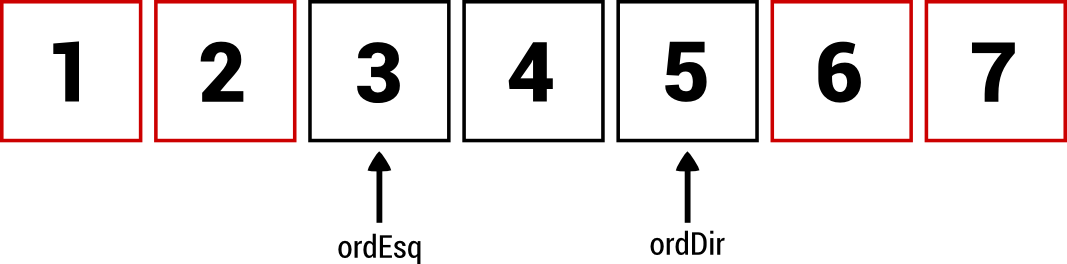
\includegraphics[scale=0.6]{img/maior.menor.algoritmo/passo5.png}
\end{figure}

\begin{figure}[h]
   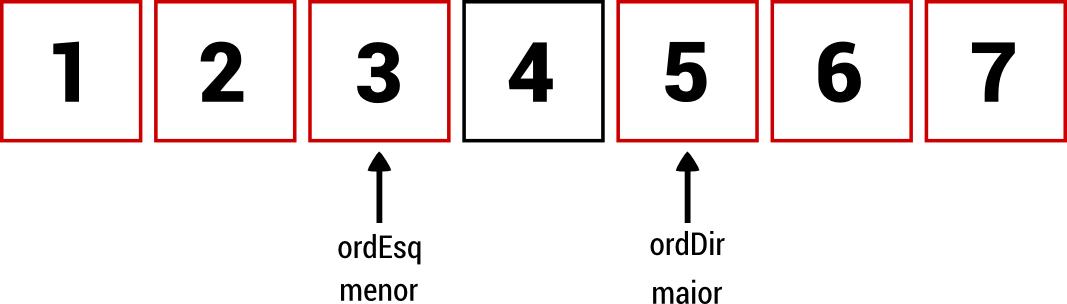
\includegraphics[scale=0.6]{img/maior.menor.algoritmo/passo6.png}
\end{figure}

Finalmente, para um \emph{array} ímpar temos que o valor de
\texttt{ordEsq} e \texttt{ordDir} são iguais. Nessa condição não restam
elementos a serem comparados.

\begin{figure}[h]
   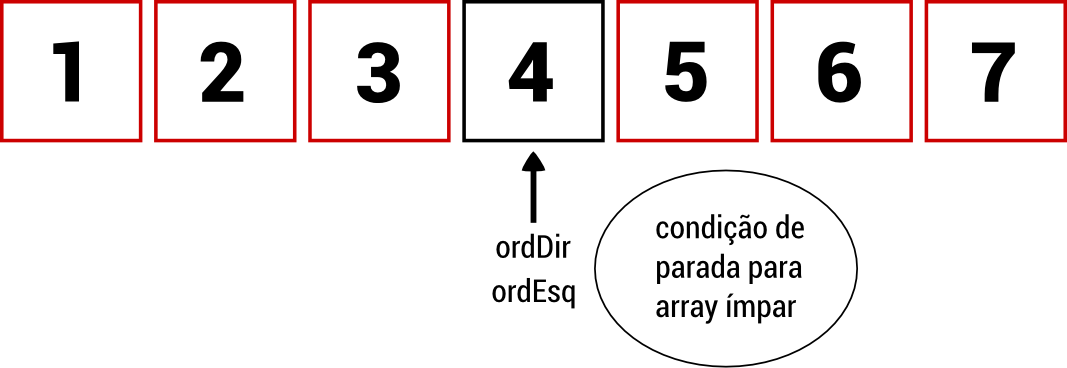
\includegraphics[scale=0.6]{img/maior.menor.algoritmo/passo7.png}
\end{figure}
